\section{Einführung}
Im Modul DMG wurde zu Übungszwecken zu relationalen Datenbanken die Uni-DB 
verwendet. Das dabei verwendete Entity-Relation Diagramm sieht folgendermassen
aus:
\begin{figure}[htbp] 
  \centering
     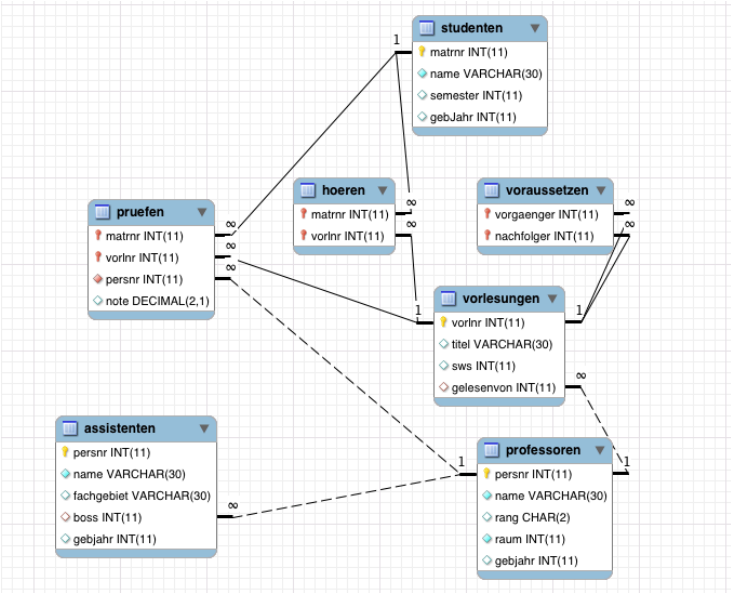
\includegraphics[width=1\textwidth]{./pictures/SQL-DB_ER_Diagramm_UNI-DB.png}
  \caption{ER-Diagramm zur Uni-DB \cite{Kaufmann2016}}
  \label{fig:uni-db}
\end{figure}
 Um mit den NoSQL Datenbanken Erfahrung zu sammeln, wird dieses Schema in die NoSQL Datenbank MongoDB überführt.
Die MongoDB als wird aus folgenden Gründen verwendet:
\begin{itemize}
  \item Wird in der Praxis eingesetzt
  \item Gute Dokumentation
  \item Kostenfrei
  \item Untstützung durch Forenuser
  \item Erste Erfahrung vorhanden
\end{itemize}
An die MonogDB wird eine Abfrage definiert, welche das selbe Resultat ergibt,
wie das folgende SQL-Query:
\begin{lstlisting}
select ProfessorName, AnzahlStudenten, SummeSWS 
from ( 
	select p.Name as ProfessorName, count(s.MatrNr) 
	as AnzahlStudenten 
		from Professoren p 
		join Vorlesungen v on v.gelesenVon = p.PersNr
		join hoeren h on h.VorlNr = v.VorlNr 
		join Studenten s on s.MatrNr = h.MatrNr 
		group by p.Name 
	) A 
join 
( 
	select p.Name as ProfessorName,  sum(SWS) 
	as summeSWS 
	from Professoren p 
	join Vorlesungen v on v.gelesenVon = p.PersNr 
	group by p.Name 
) B using(ProfessorName)
\end{lstlisting}

